% Chapter 1

\chapter{Introduction} % Main chapter title

\label{Chapter1} % For referencing the chapter elsewhere, use \ref{Chapter1} 

\lhead{Chapter 1. \emph{Introduction}} % This is for the header on each page - perhaps a shortened title

%----------------------------------------------------------------------------------------

\section{Overview}

Traditional voting systems in use across elections around the world rely on paper ballots. The voters are expected to cast their votes, in person at a polling booth, with officials from an overseeing body ensuring a fair conduct. A large number of places also allow voters to send in their votes by post. In a paper ballot based setting, the most time consuming part is the counting and reconciliation of ballots.

Evoting systems aim to provide an efficient replacement for paper ballots. Efficiency improvements aside, it is essential that the evoting systems provide transparency and anonymity properties during the course of the election. These properties may include:

\begin{enumerate}
\item Identification of the voter
\item Coercion resistance
\item Not allowing anyone to figure out who a person voted for
\item Allowing the voter to ensure his/her vote is cast as intended, i.e. no adversary has changed his/her vote while it was being cast (cast-as-intended)
\item Allowing the voter to ensure his/her vote is actually recorded (recorded-as-cast)
\item Allowing all stakeholders to verify if the evoting system has counted the ballots properly (count-as-recorded)
\end{enumerate}

Another desirable property for an evoting system would be to have it decentralised, i.e. no single entity should be able to perform operations on the data store. All modifications should require a threshold majority to be accepted. This prevents a single entity from manipulating the election.

Having laid down some desirable properties of evoting systems, we now focus our attention to the current evoting application at EPFL, discuss its limitations and propose a new evoting system which satisfies a subset of the aforementioned properties making it suitable for conducting elections in EPFL.
%----------------------------------------------------------------------------------------

\section {Background}

EPFL conducts elections for positions at Faculty/School Councils and School Assembly every year \cite{assemblyEPFL}. The current election system, uses InForm \cite{inform}, a questionnaire service provided by Vice Presidency for Information Systems (VPSI) \cite{vpsi}. Inform's voting module consists of a centralised application written in PHP which uses MySQL as its data store. It does not encrypt the ballots but ensures voter privacy by not associating user information with the ballots. The system logs if a person has voted before to prevent more than one ballot being cast by the user. Once the election is over, the central server then performs an aggregation of all the votes recorded and displays the final count. InForm also allows exporting the ballots as a CSV file to allow a manual count of the ballots.

The centralised nature of the application means that the administrator(s) with access to the deployment server hold complete control over the election. Even though no user information is associated with the ballot, the timestamp to log a user's vote can be used to associate a user to a particular ballot thereby affecting voter privacy. This also prevents auditing the aggregation of ballots in the case where an adversary manages to cast fake ballots in the system. Any attempts to reconcile the votes would lead to leaking the voter privacy of all users associated with the election.

In light of the aforementioned limitations of InForm, we propose an implementation of an auditable and distributed evoting system, which builds on the work of Andrea Caforio \cite{andrea} and Etienne Bonvine \cite{etienne} which they did as a part of the Masters and Bachelors project respectively. The voting procedure briefly works as follows:

\begin{figure}[htpb]
  \centering
    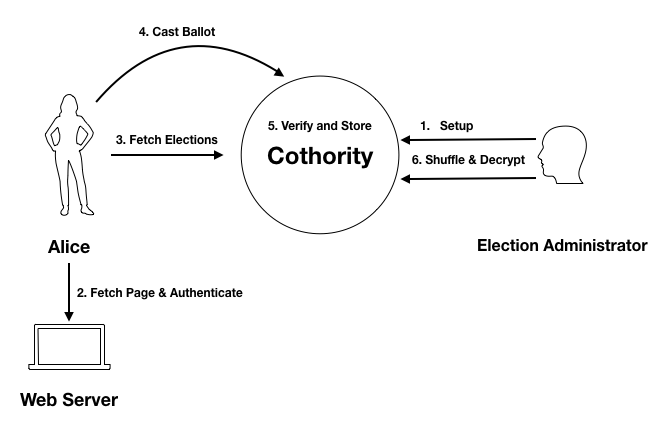
\includegraphics[scale=0.4]{Figures/Overview.png}
    \rule{35em}{0.5pt}
  \caption[Voting Procedure]{Voting Procedure}
  \label{fig:Voting Procedure}
\end{figure}

\begin{enumerate}
\item An election administrator sets up an election with a list of candidates and the users allowed to participate in the election. For this example, let's assume Alice is allowed to vote in one of the elections. Setting up an election happens in a distributed manner with each participating server generating a secret. An aggregate public key is generated using these secrets and it may be used to encrypt messages on client side.
\item Alice visits the frontend client using a browser. The client checks for the presence of a signature in the browser's localStorage \cite{localStorage}, verifying her identity or redirects Alice to an authentication endpoint in its absence.
\item After successful authentication, Alice can see all the elections she is eligible to participate in.
\item Alice may cast as many ballots as she wishes for each election she is allowed to participate in. The ballot is encrypted in the browser before being sent to the backend for storage.
\item Alice's encrypted ballot is then published in a distributed ledger which is accessible to everyone.
\item After the election ends, the election administrator may initiate mixing of all ballots, where the last cast ballot by each user is taken in account and shuffled by a threshold number of participating nodes in the election, one node at a time. The shuffle is stored in the distributed ledger only if a threshold number of nodes can verify its integrity.
\item The last shuffle is then decrypted by each participating node using its share of the secret.
\item Alice or any external auditor may then see the final tally of votes by reconstructing the decryption shares of a threshold number of nodes and counting the decrypted ballots.
\end{enumerate}

It is important to note that the evoting system only encrypts the user's ballots but not their identity. It is therefore possible to ensure if a user voted or not (recorded-as-cast) and the encryption ensures no one can ascertain which candidate(s) the user voted for. The current implementation however does not allow the voter to ensure if their vote is cast-as-intended.

Having introduced the system in brief, we now turn our attention to the system architecture and implementation details